\section{Radio Frequency Interference (RFI)}

Unfortunately, as the survey has progressed, we have been increasingly beset by terrestrial, satellite and aircraft interference (see Figure~\ref{fig:intensity}). Aircraft interference is sporadic enough in nature to flag out, but satellite and terrestrial interference is, however, more troublesome (see \fign{fig:intensity}). The effect on the data is noticeable up to 50$^{\circ}$ elevation, making post-measurement removal very difficult, if not impossible.

The RFI consists of both in band and out of band signals. Different approaches have been adopted to deal with them. We have designed a set of appropriately narrow band notch filters to deal with the in-band RFI (see \appen{sec:filterDesign} for details), and have cascaded an additional set of the original bandpass filters to combat out of band RFI.

 The resulting change of the passband can be seen in \fign{fig:passbands}. The effect on data quality (\fign{fig:intensityFiltering}) is noticeable with the 0.25s/pixel integration period used to produce these scans.



\begin{figure}
 \centering
\subfloat[][The C-BASS pass band before installing any additional filtering]{
 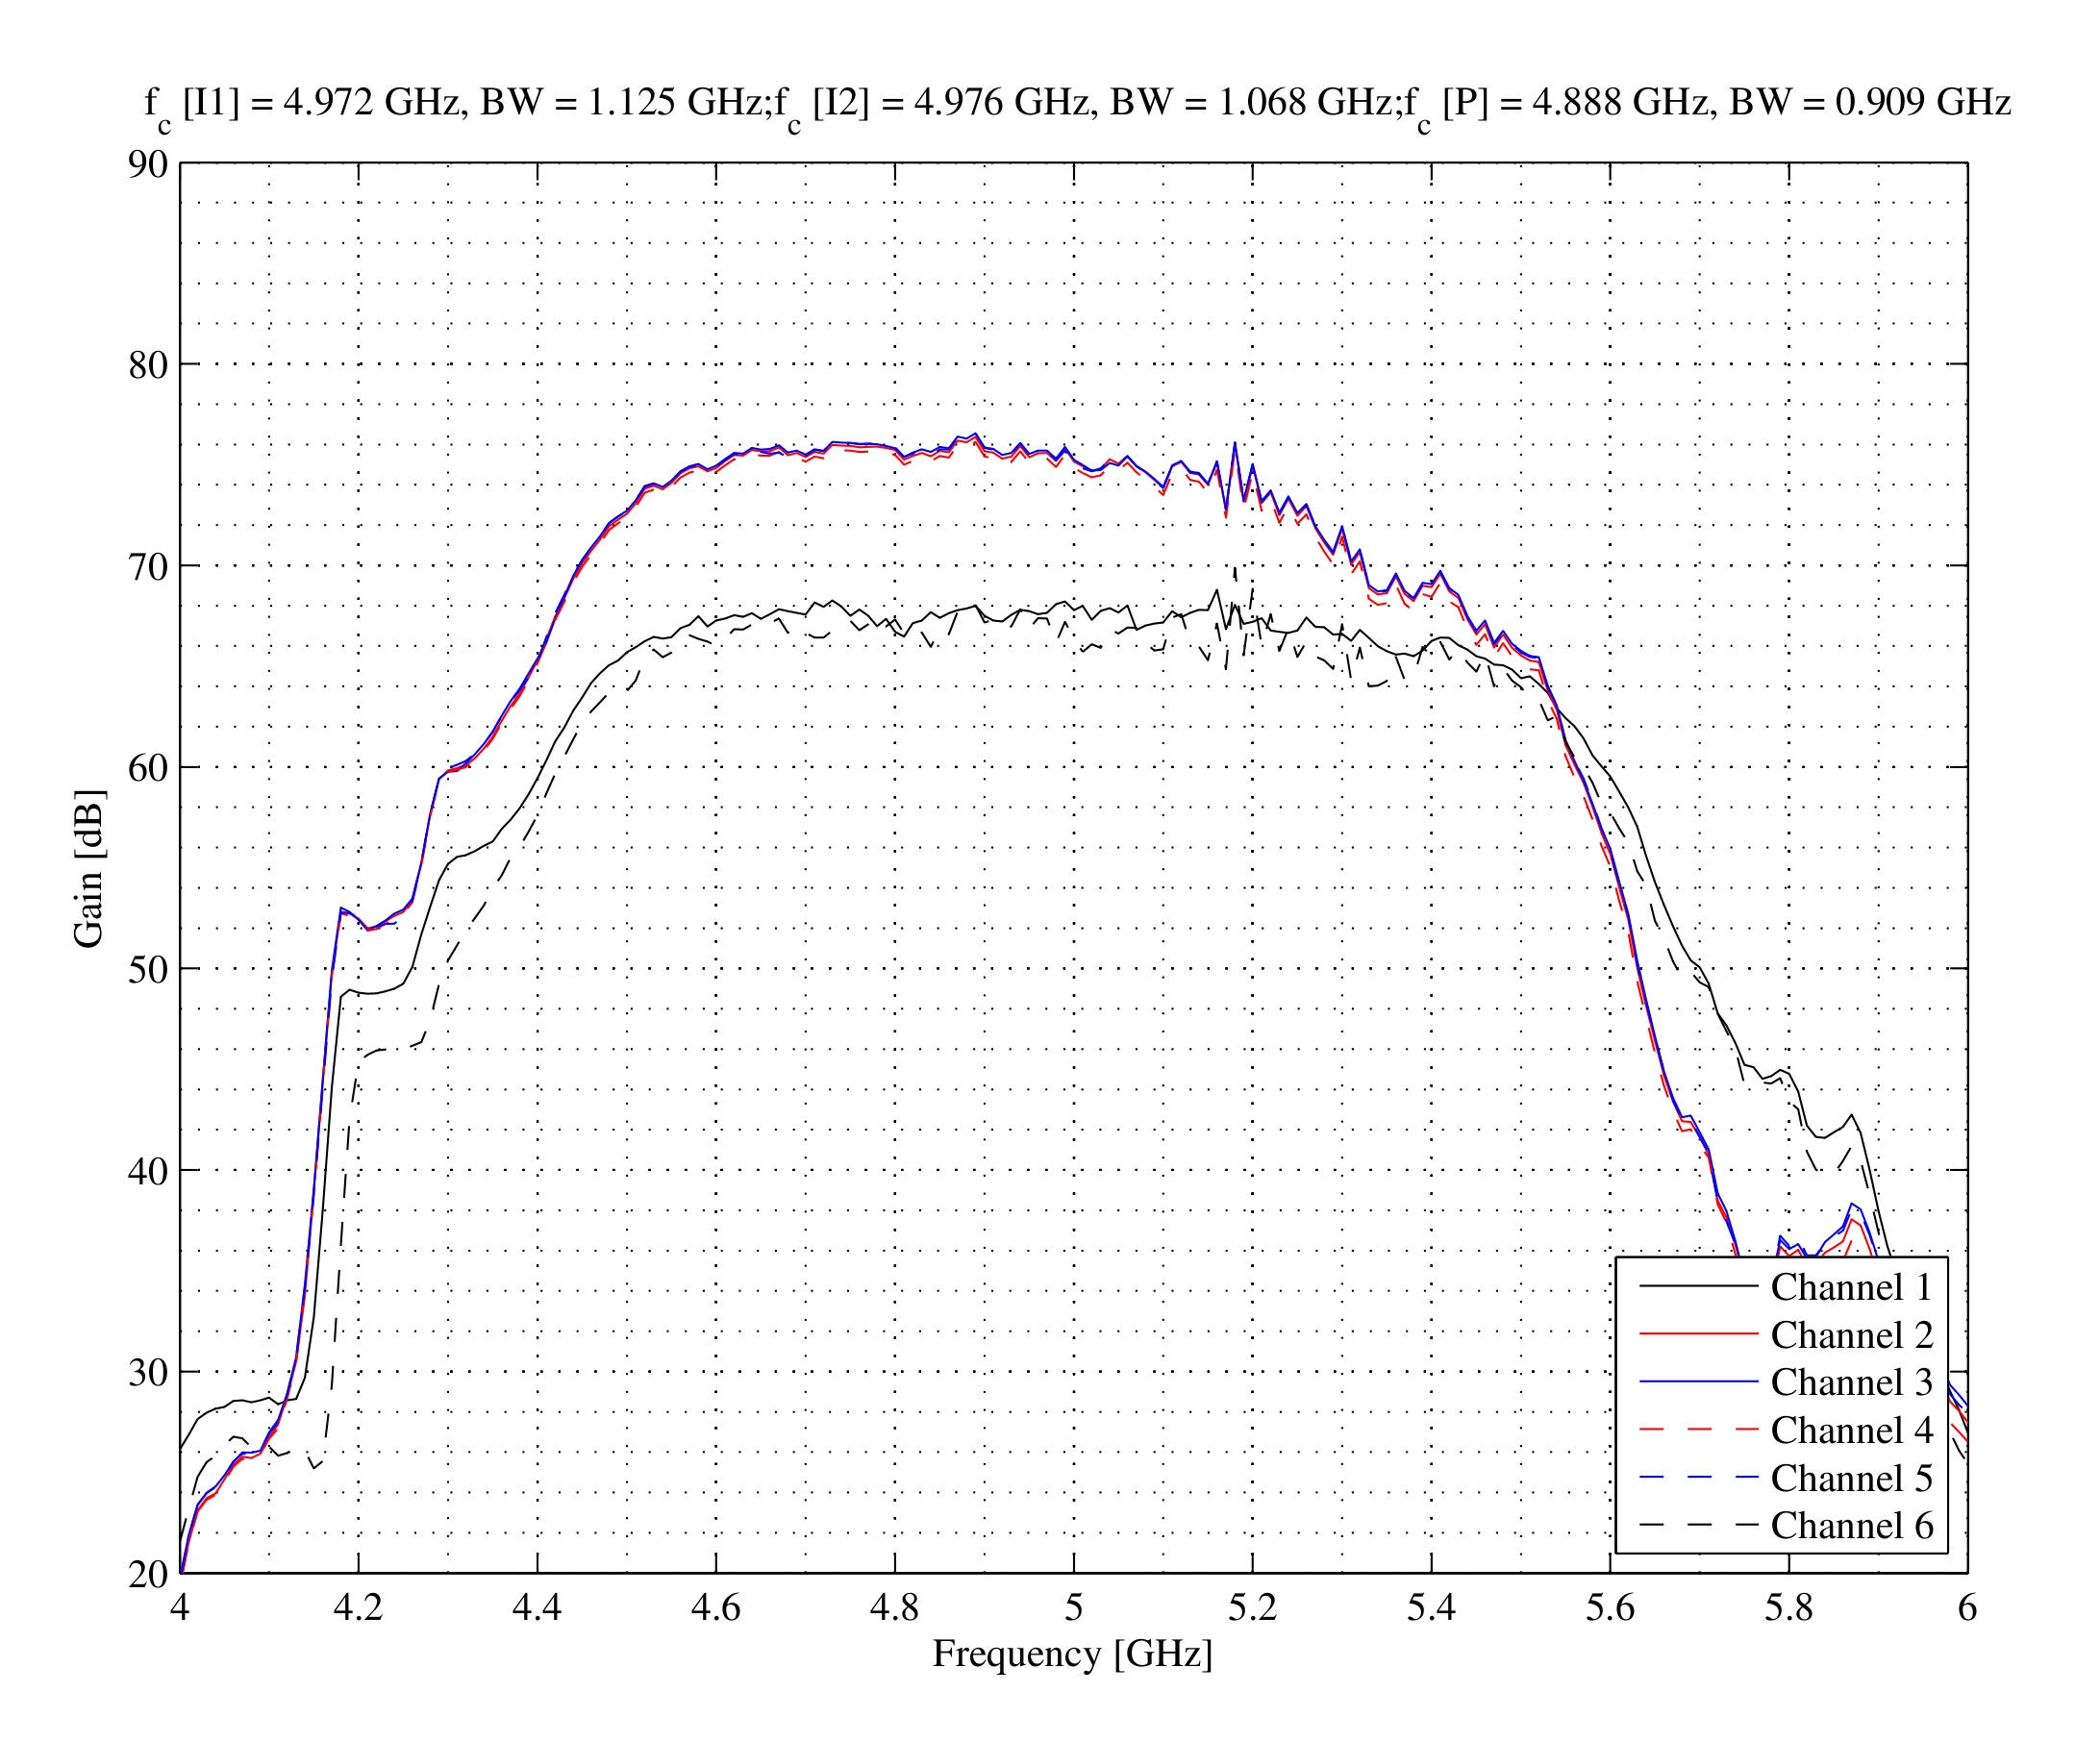
\includegraphics[height=0.4\textheight]{./images/NotchFilter/firstpassband.png}
}\\
\subfloat[][The C-BASS pass band after installing the Notch filters and additional Band pass filters]{
 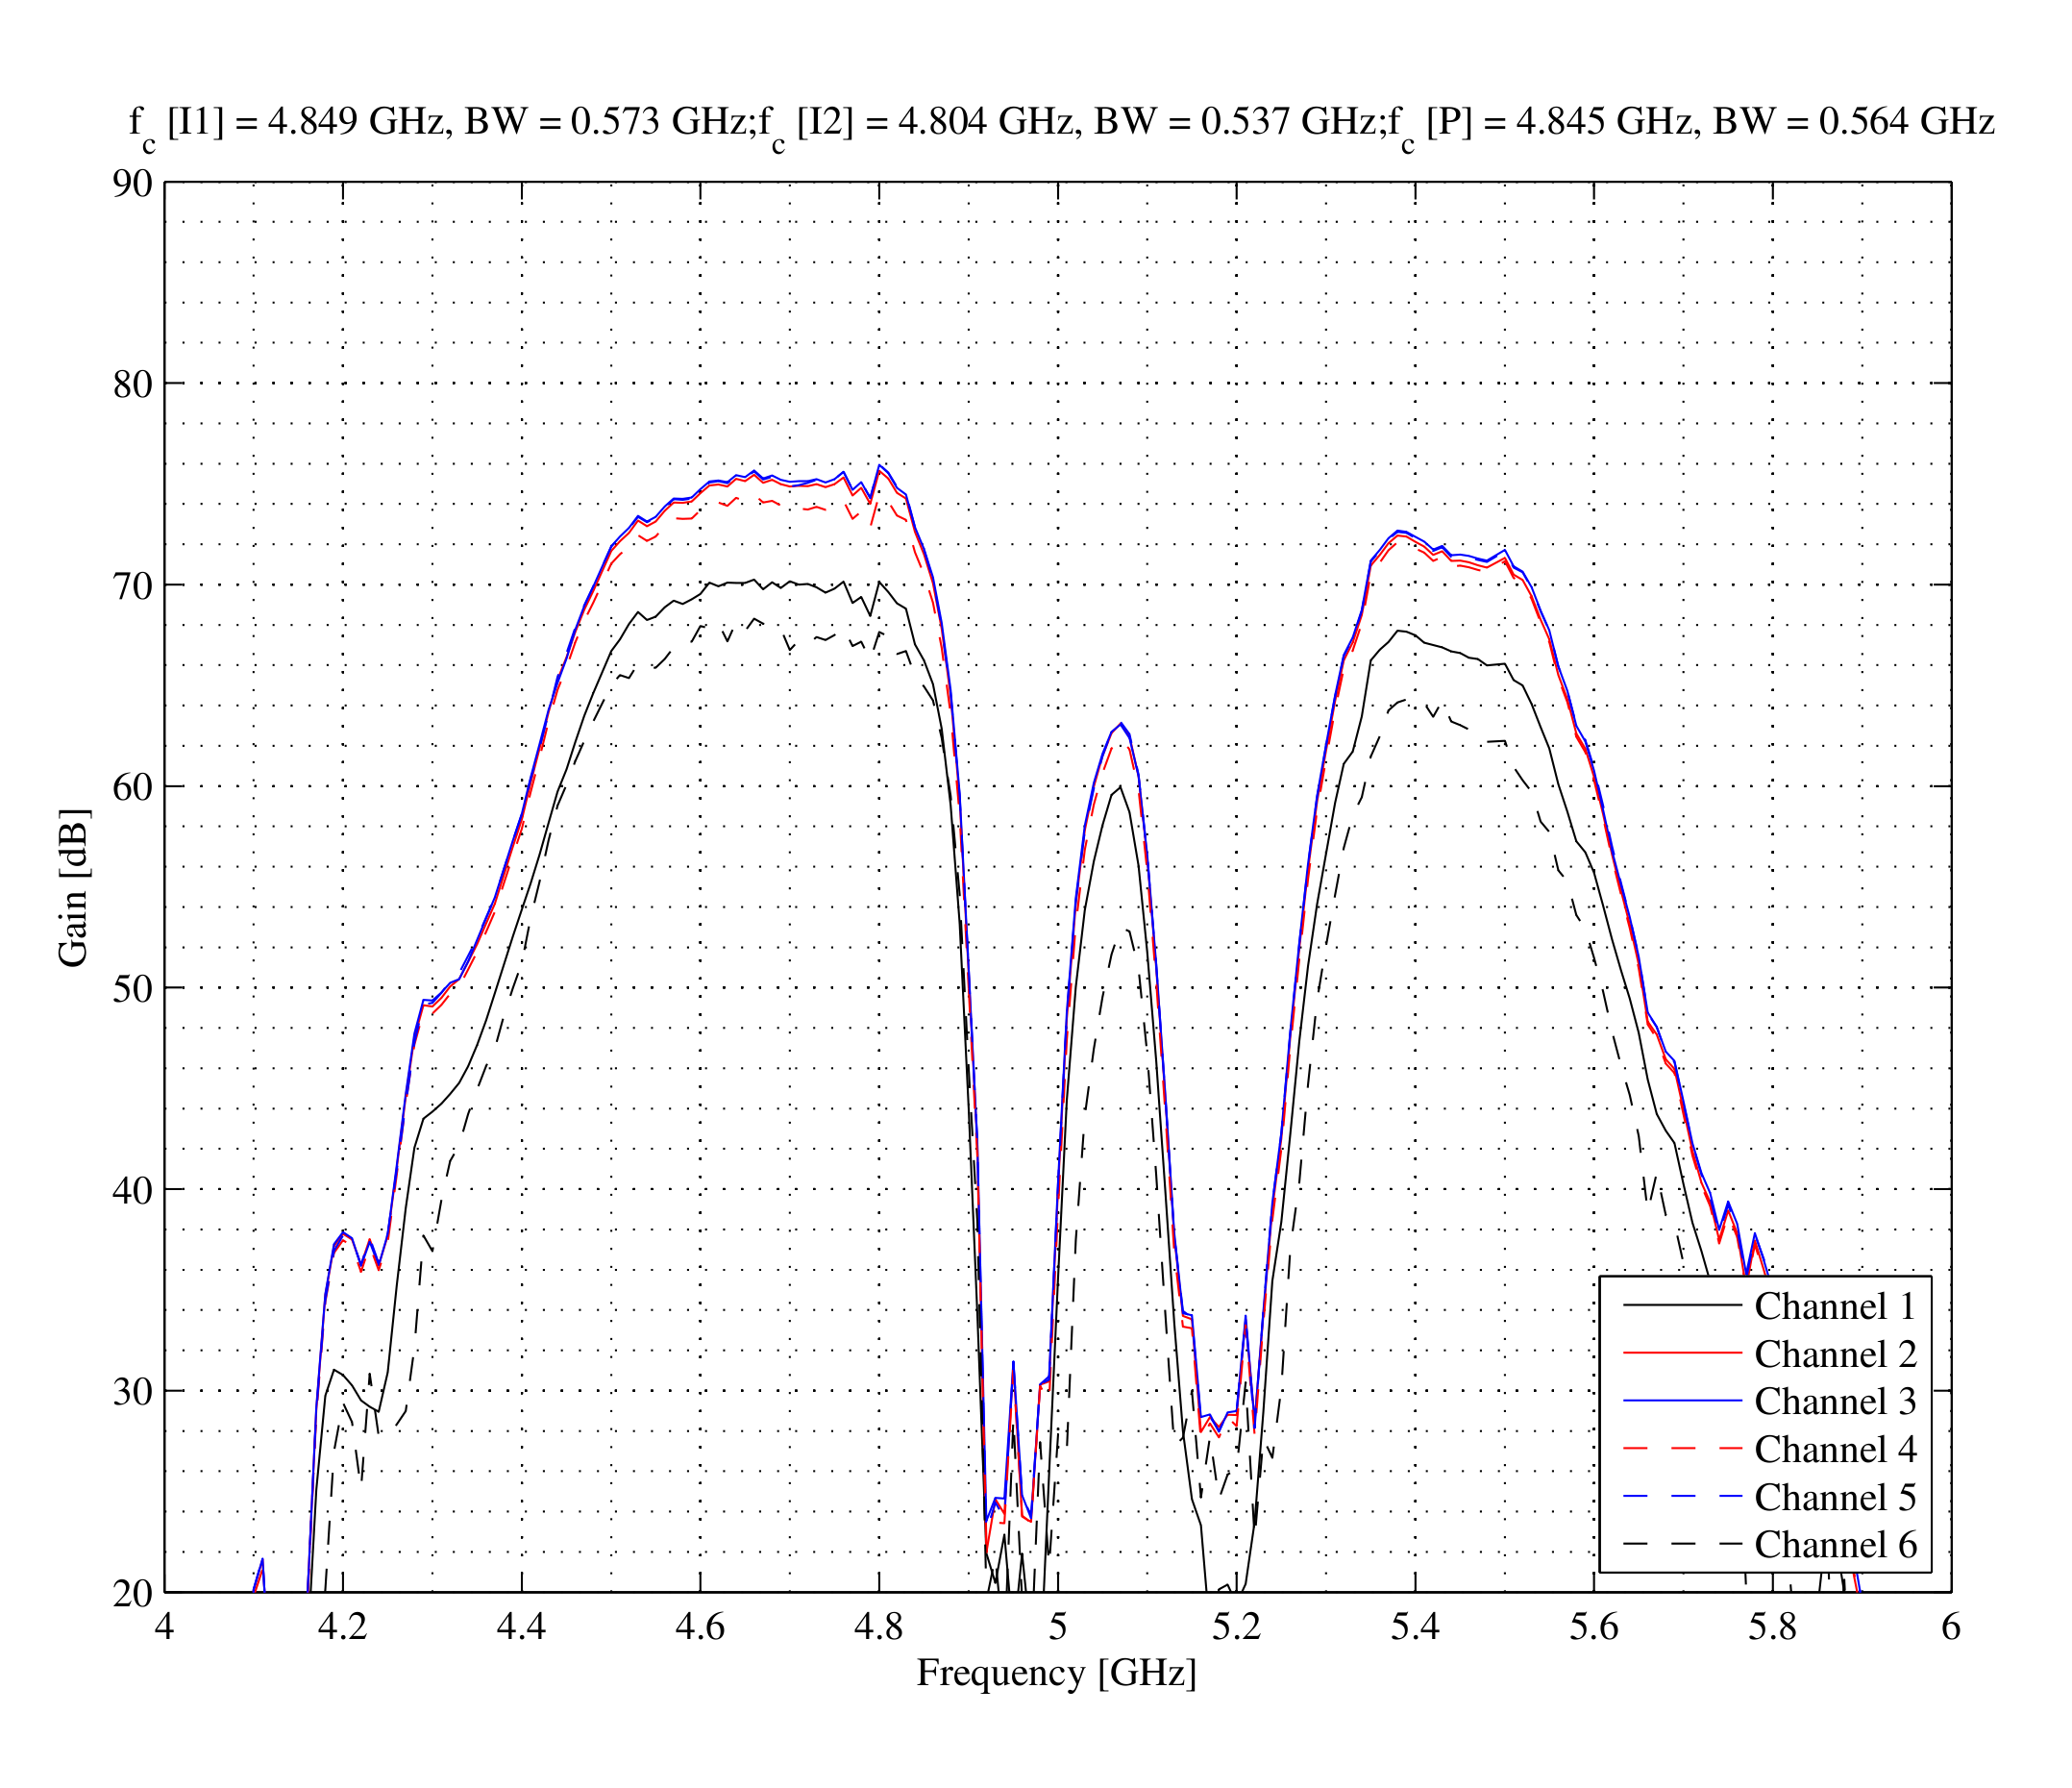
\includegraphics[height=0.4\textheight]{./images/NotchFilter/finalpassband.png}
}
 % firstpassband.pdf: 612x792 pixel, 72dpi, 21.59x27.94 cm, bb=
 \caption{C-BASS passband changes}
 \label{fig:passbands}
\end{figure}

\begin{figure}[ht]
 \centering
 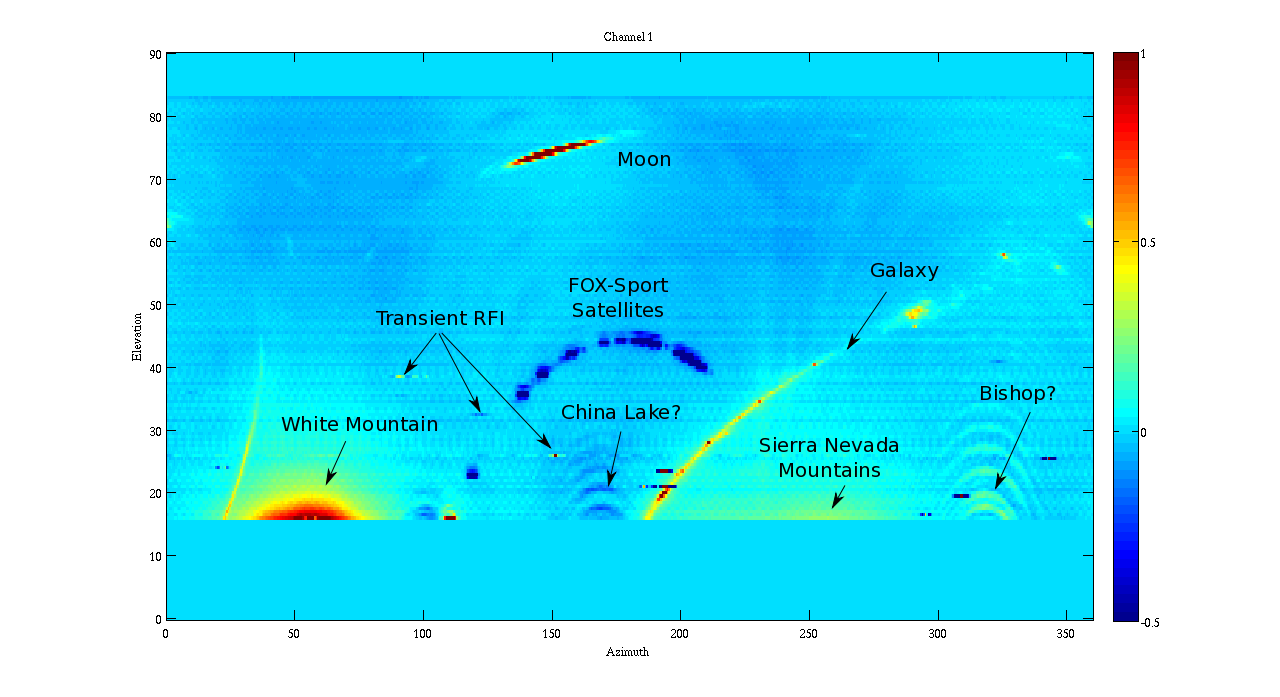
\includegraphics[width=\textwidth]{./images/NotchFilter/altazmapannotated.png}
 % altazmapi.png: 1280x701 pixel, 90dpi, 36.13x19.79 cm, bb=0 0 1024 561
 \caption{Annotated Intensity map (courtesy Oliver) of the sky as seen by the Owens Valley C-BASS antenna. Note the elevation extent of the diffraction patterns seen as a result of the terrestrial radiation }
 \label{fig:intensity}
\end{figure}


\begin{figure}
 \centering
\subfloat[][Sky before the installation of notch filters. Note the diffraction patterns produced by strong RFI sources detected in the antenna sidelobes]{
 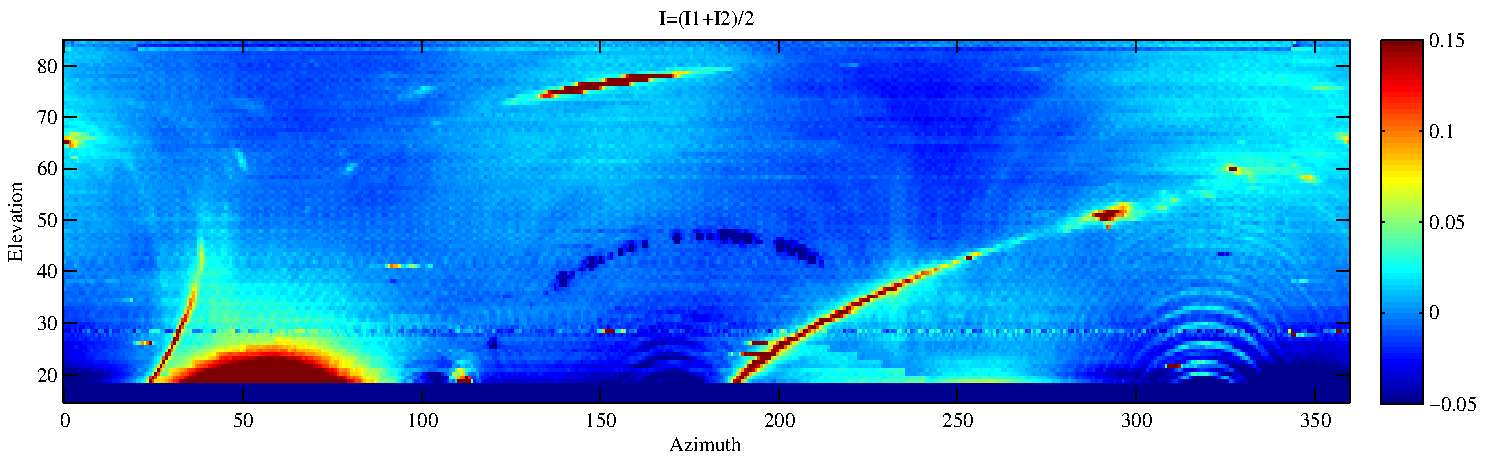
\includegraphics[height=0.25\textheight]{./images/NotchFilter/IntensityChannelBeforeNotch.pdf}
}\\
\subfloat[][Sky after the installation of notch filters. All terrestrial RFI aside from a strong source to the South ($180^{\circ}$~Azimuth) has been removed ]{
 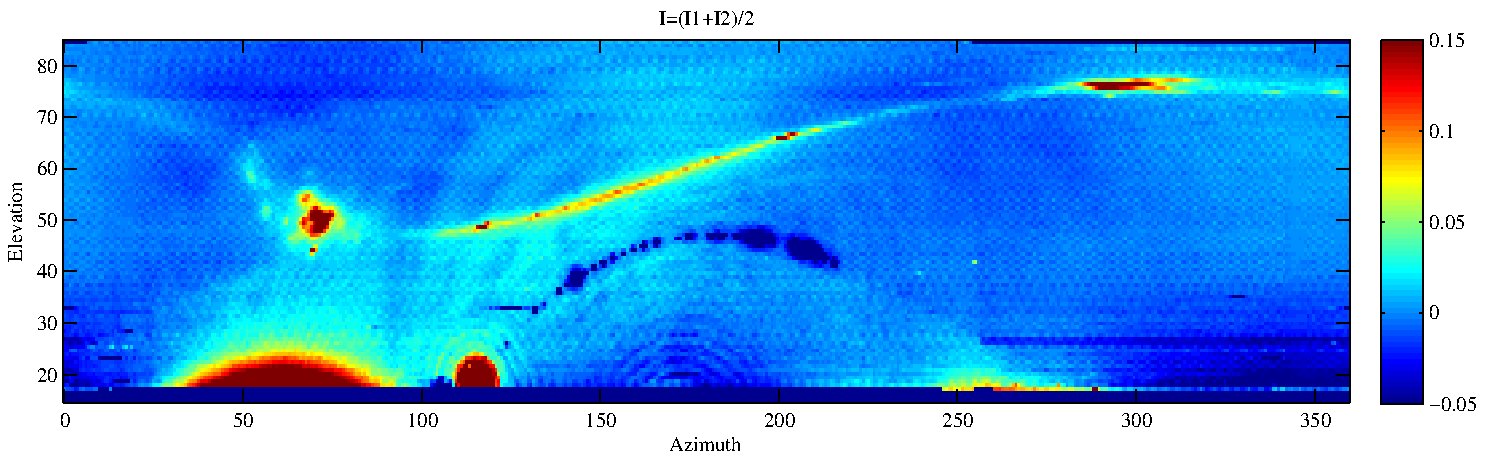
\includegraphics[height=0.25\textheight]{./images/NotchFilter/IntensityChannelAfterNotch.pdf}
}\\
\subfloat[][Sky after the installation of notch filters and additional band pass filters. All terrestrial radiation removed, and geostationary satellites are no longer visible]{
 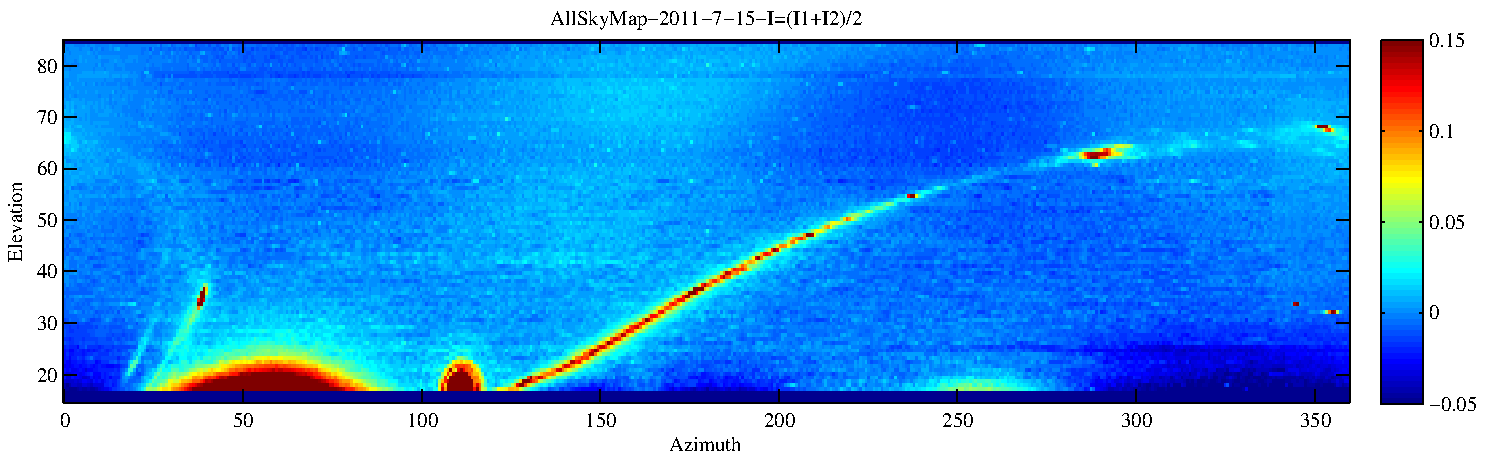
\includegraphics[height=0.25\textheight]{./images/NotchFilter/IntensityChannelAfterBPFandNotch.pdf}
}
\caption{Installing additional filtering: These images show the dramatic improvement in data quality brought about by the addition of notch filters and additional band defining filters in the C-BASS RF path}
\label{fig:intensityFiltering}
 % IntensityChannelBeforeNotch.pdf: 713x220 pixel, 72dpi, 25.15x7.76 cm, bb=
\end{figure}


\begin{figure}
 \centering
\subfloat[][Radio Frequency Interference as captured by a spectrum analyser attached to the output of the C-BASS cryostat. We think the 4.79~GHz spike is sporadic and does not require filtering]{
 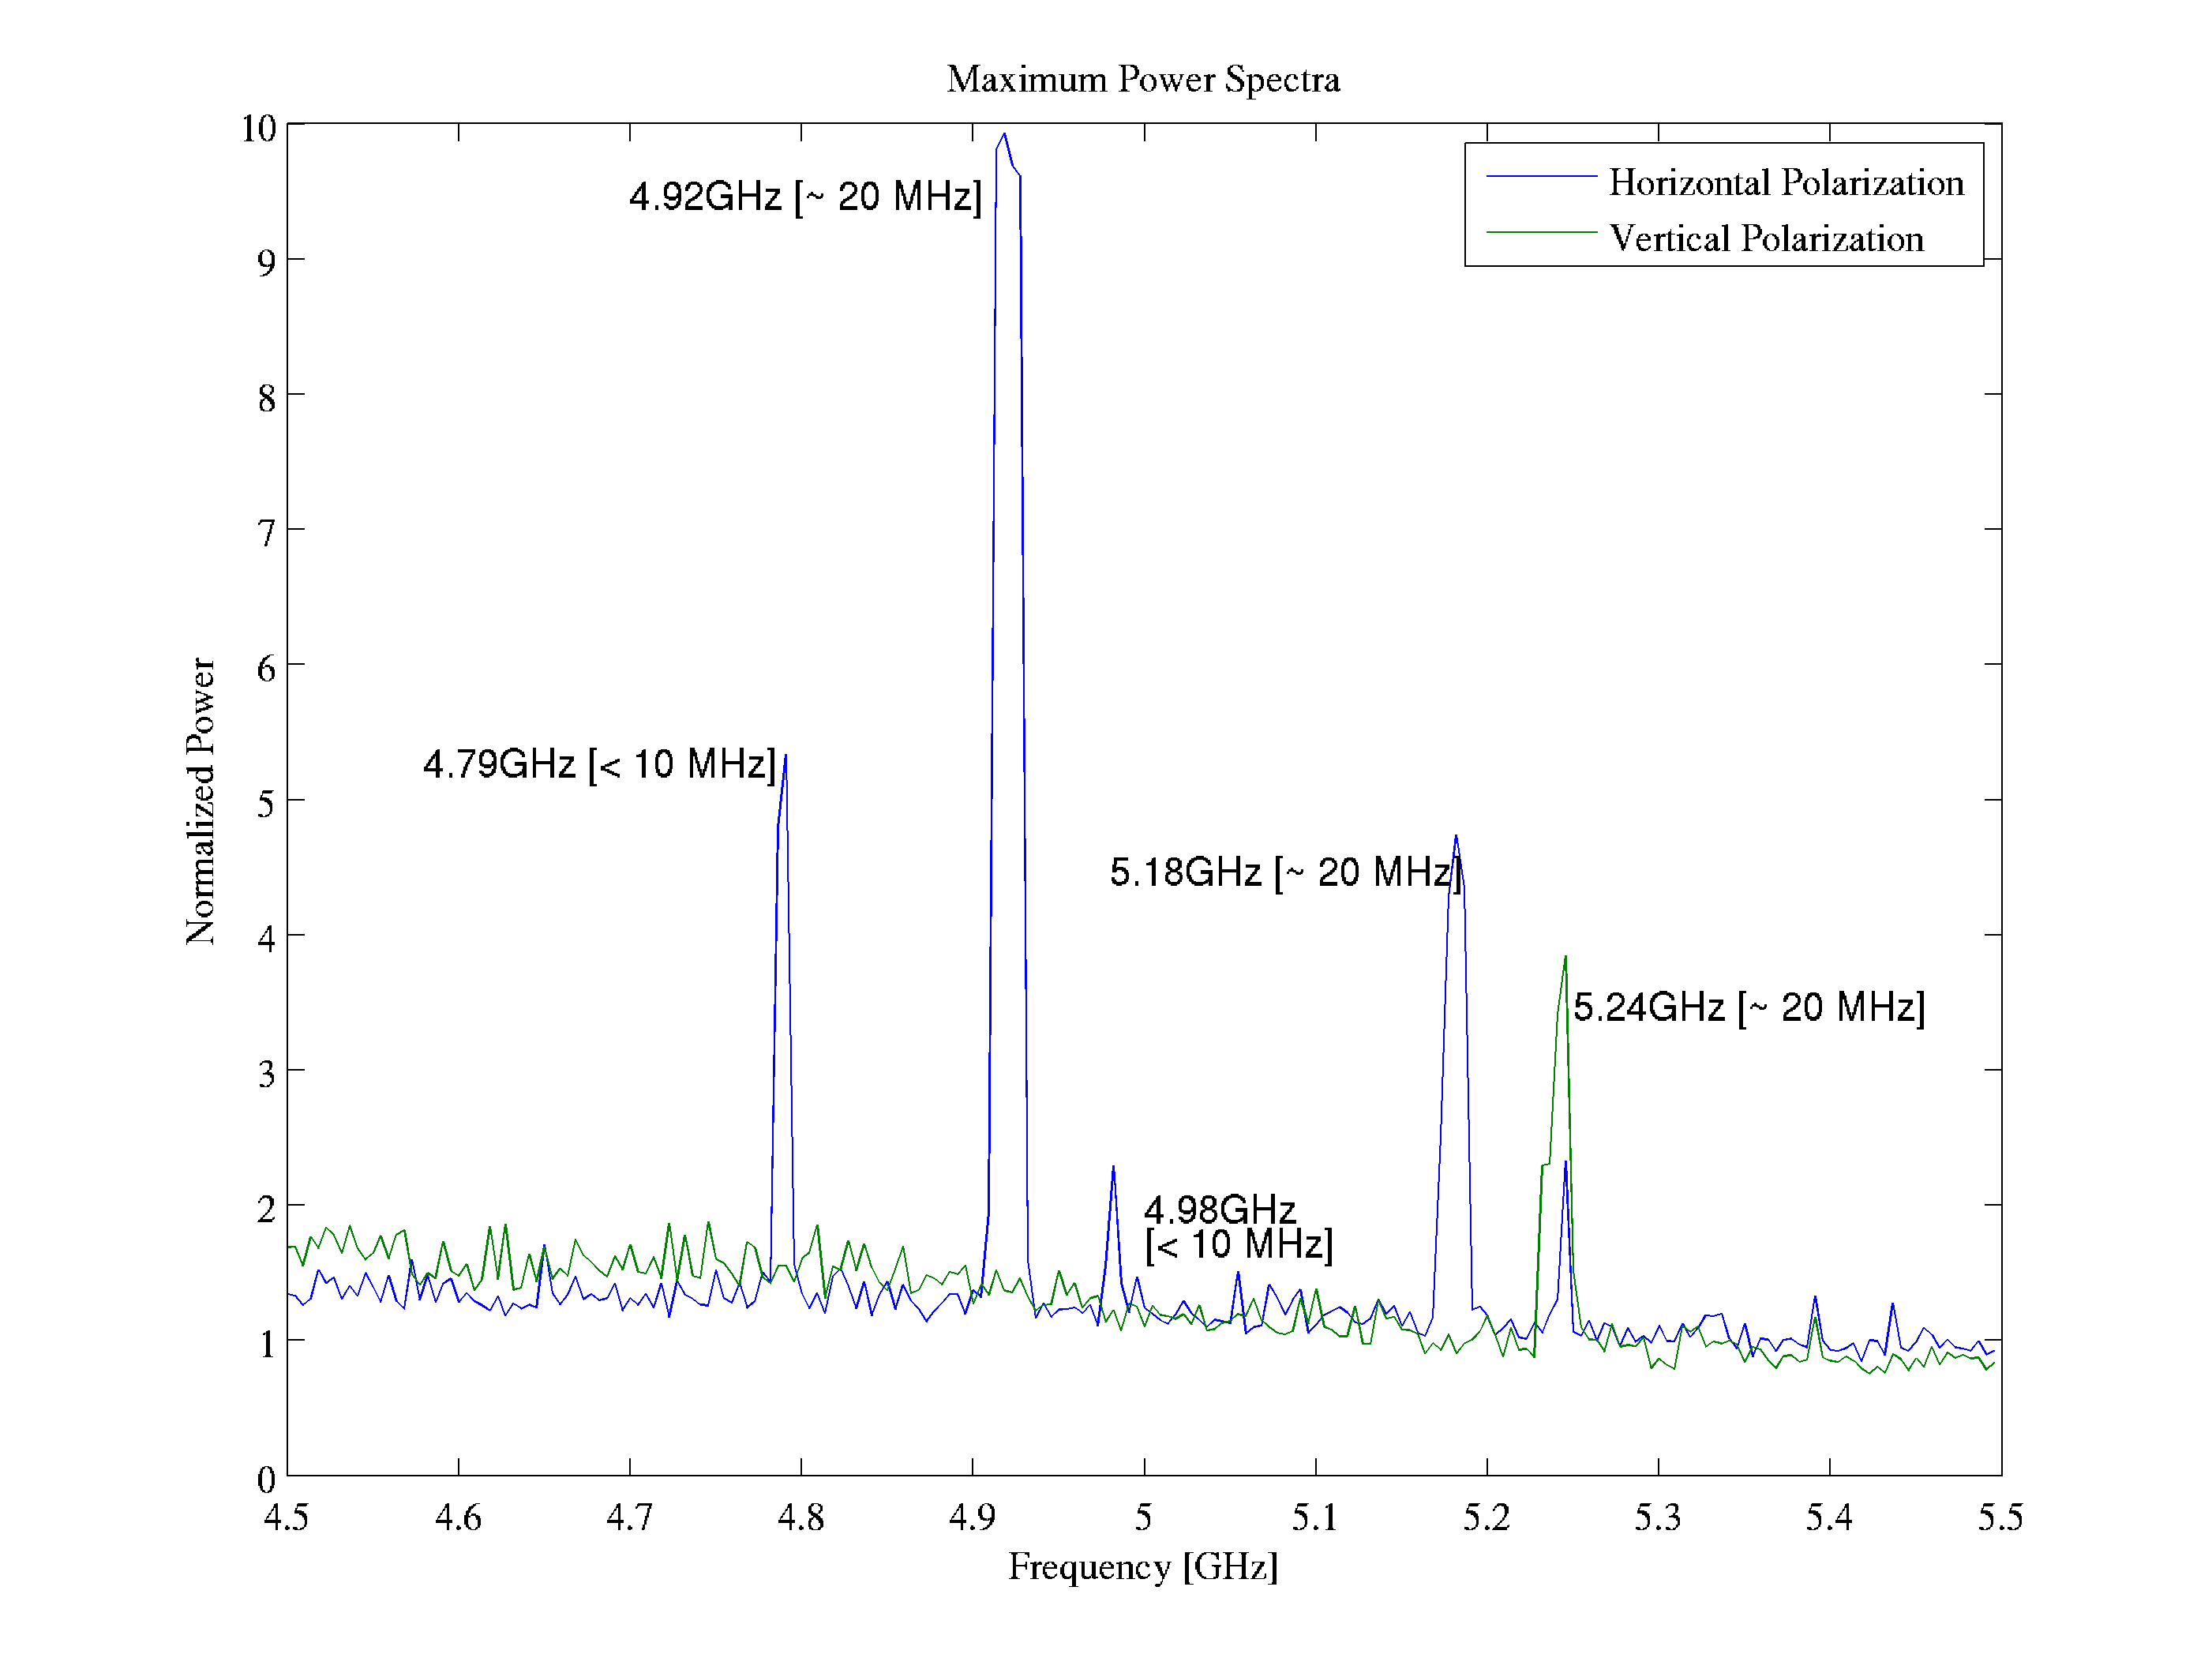
\includegraphics[height=0.4\textheight]{./images/NotchFilter/RFI/norm_max_rfi.png}
}\\
 % norm_max_rfi.png: 2802x2100 pixel, 350dpi, 20.33x15.24 cm, bb=0 0 576 432
 \subfloat[][Power Spectrum of geostationary satellites]{
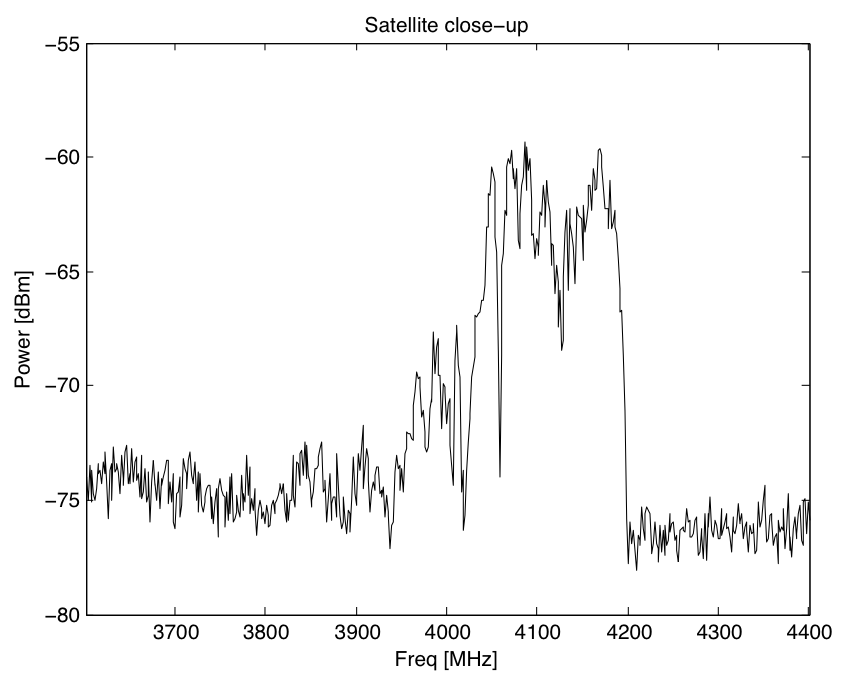
\includegraphics[height=0.4\textheight]{./images/NotchFilter/RFI/figs-satellite.png}}
\caption{}
 \label{fig:RFImaxHold}
\end{figure}




\clearpage
% \begin{figure}
%  \centering
%  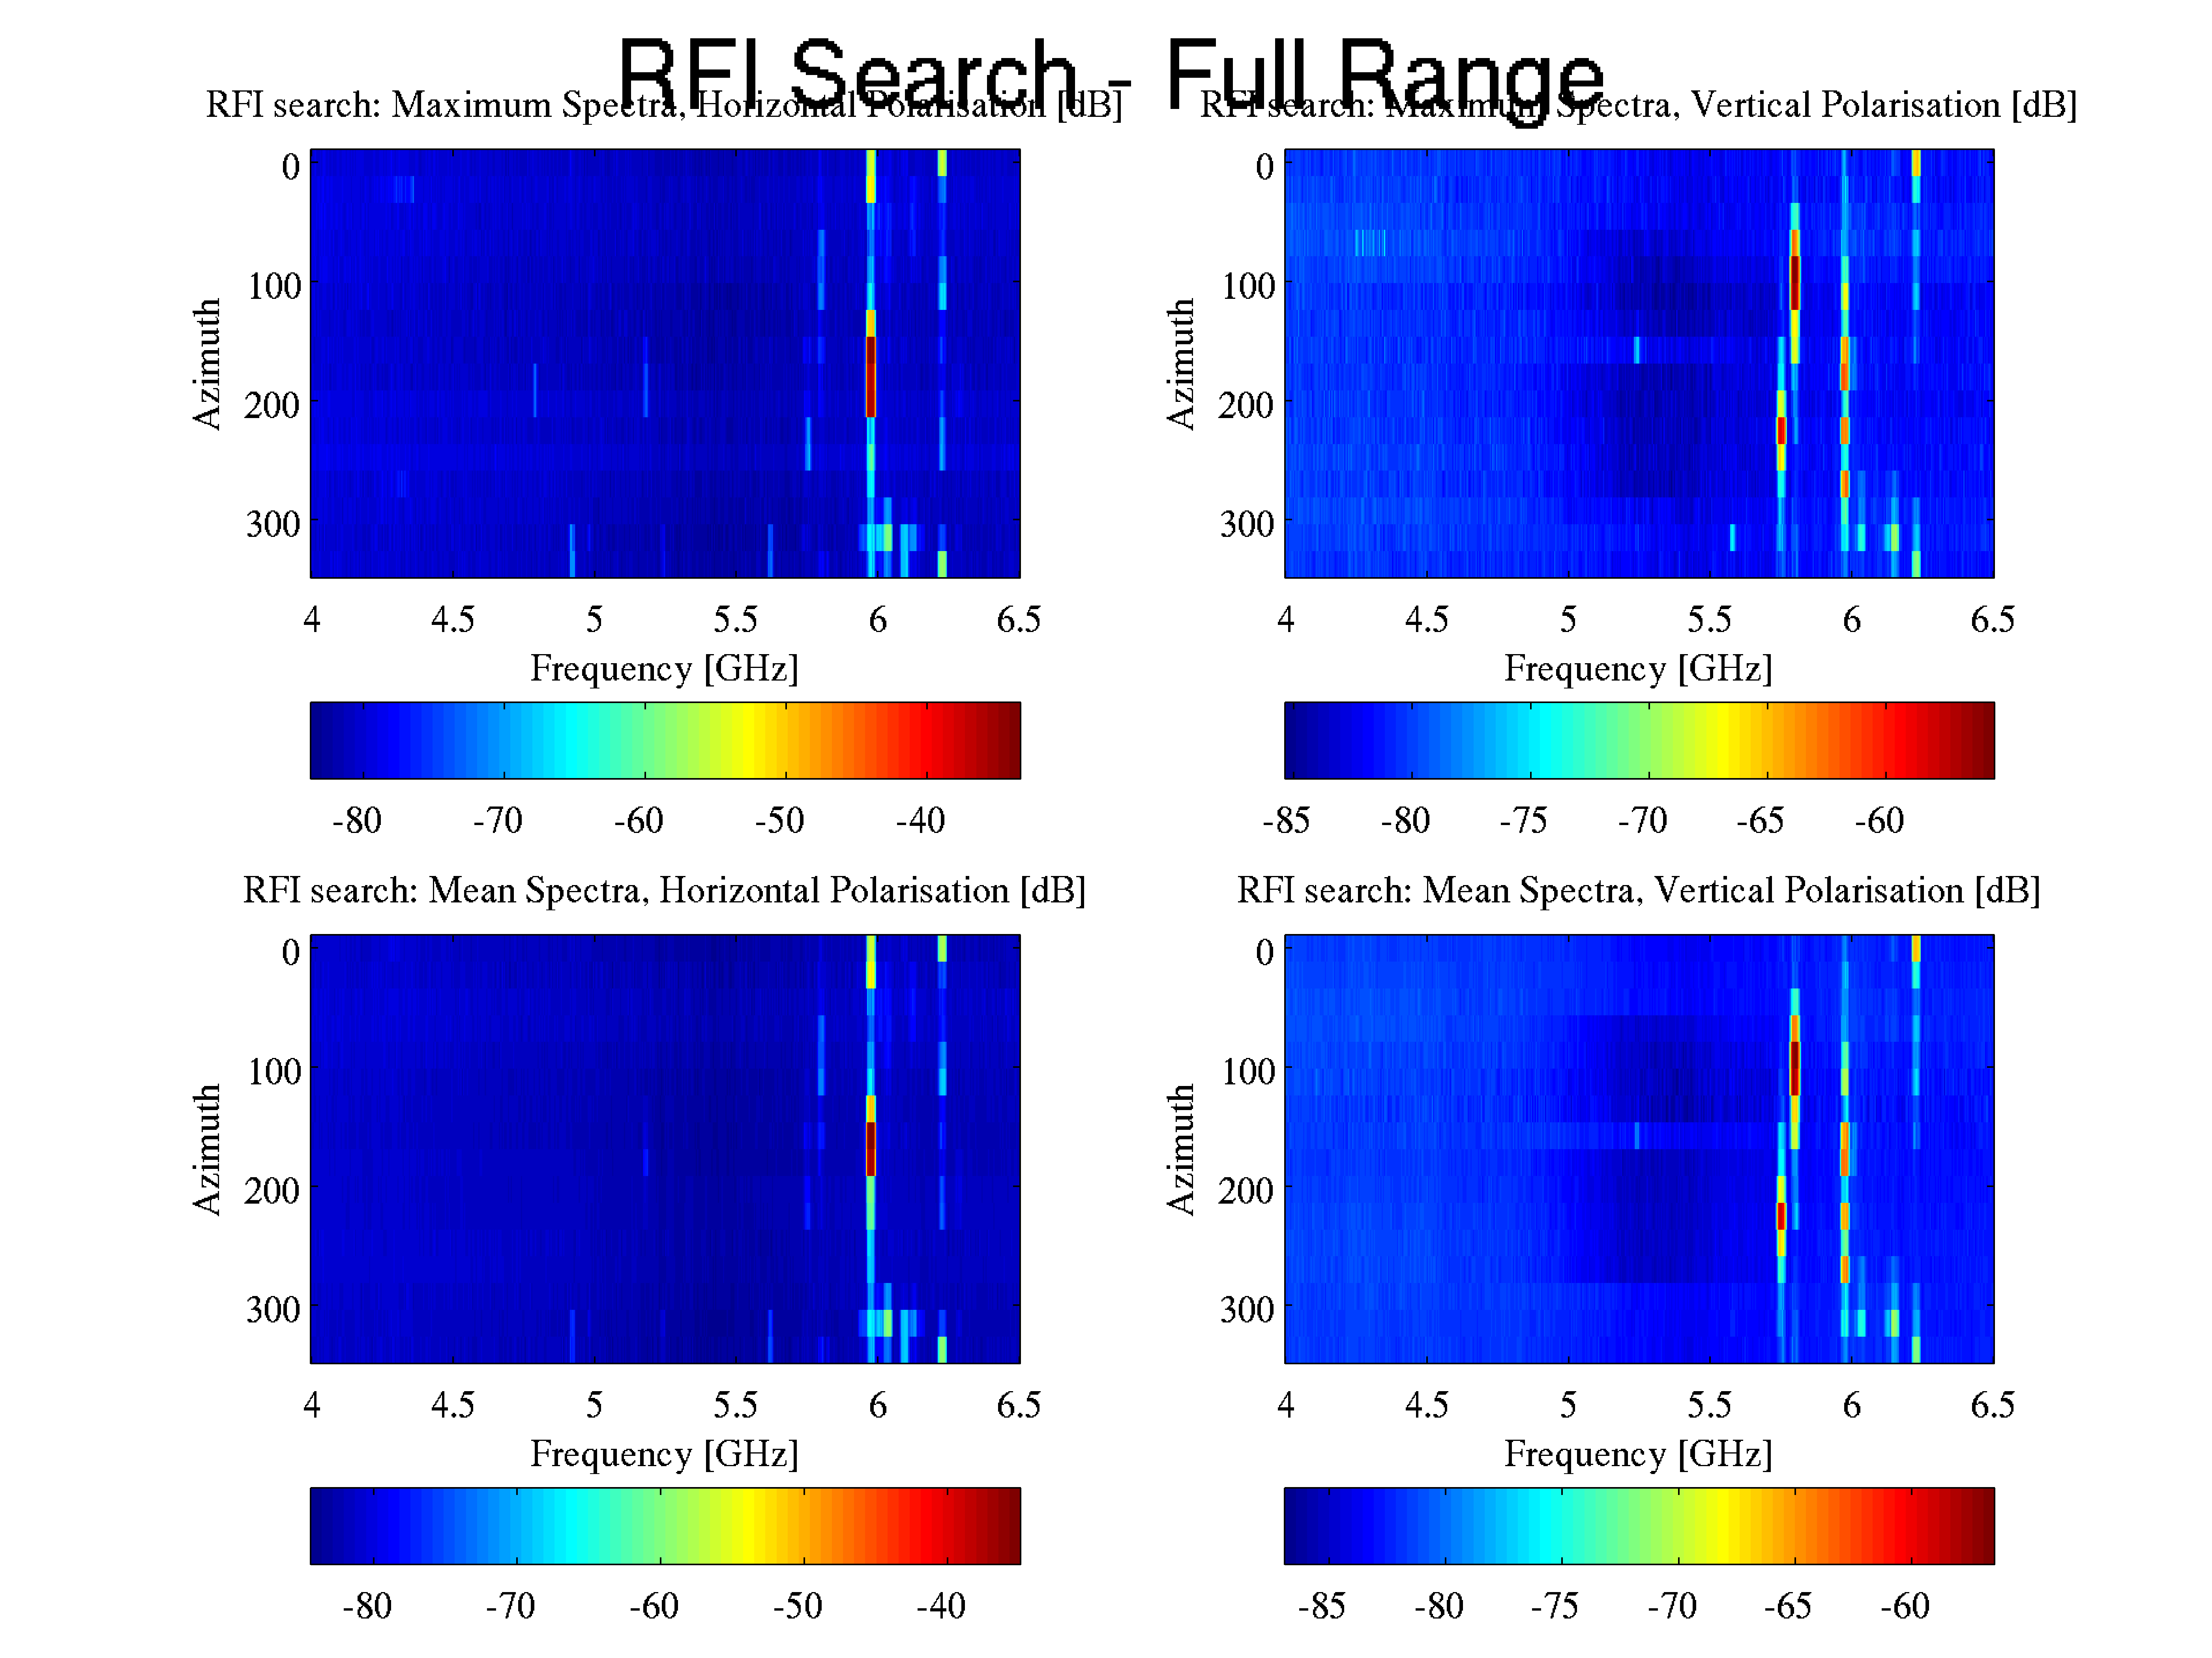
\includegraphics{./images/NotchFilter/RFI/rfi_full_range.png}
%  % rfi_full_range.png: 5605x4200 pixel, 700dpi, 20.34x15.24 cm, bb=0 0 577 432
%  \caption{Radio Frequency Interference as seen at Owens Valley with directionality}
%  \label{fig:RFI}
% \end{figure}


